\documentclass[aspectratio=169]{beamer}
\usepackage[T1]{fontenc}
\usepackage[default]{sourcesanspro}
\usepackage{newtxsf}
\usepackage{hyperref}
\usepackage{latexsym,amsmath,xcolor,multicol,booktabs,calligra}
\usepackage{graphicx,pstricks,listings,stackengine}
\graphicspath{{./figures/}}
\usepackage{lipsum}
\usepackage{wrapfig}
\usepackage{url}
\usepackage{subcaption}
\usepackage{listings}
\usepackage{minted}
\setminted{fontsize=\footnotesize}
\usepackage{fontawesome5}

\usepackage{etoolbox}
%\usefonttheme[onlymath]{serif}

\author{Yan Lin}
\title{AI Systems \& Infrastructure}
\subtitle{Module A.4: AI API Servers}
\institute{%
    \href{https://www.yanlincs.com}{www.yanlincs.com}
}
\date{September 1st, 2026}
\usepackage{AAU}
% \AtBeginSection{}  % Remove section title slides
\AtBeginSubsection{}  % Remove subsection title slides
\setbeamertemplate{navigation symbols}{}  % Remove bottom nav tools
% \setbeamertemplate{headline}{}  % Remove top navbar

% defs
\def\cmd#1{\texttt{\color{red}\footnotesize $\backslash$#1}}
\def\env#1{\texttt{\color{blue}\footnotesize #1}}
% set colors
\definecolor{aauyellow}{RGB}{167, 131, 55}
\definecolor{aaublue}{RGB}{32, 26, 78}
\definecolor{aaured}{RGB}{152, 43, 28}
\definecolor{textgrey}{RGB}{60, 60, 60}

\setbeamercolor{normal text}{fg=textgrey}
\usebeamercolor[fg]{normal text}

\def\emphasis#1{{\color{aaured}\textbf{#1}}}
\renewcommand{\thefootnote}{}


\lstset{%
    basicstyle=\ttfamily\small,
    keywordstyle=\bfseries\color{deepblue},
    emphstyle=\ttfamily\color{deepred},    % Custom highlighting style
    stringstyle=\color{deepgreen},
    numbers=left,
    numberstyle=\small\color{halfgray},
    rulesepcolor=\color{red!20!green!20!blue!20},
    frame=shadowbox,
}

%- --- --- --- --- --- --- --- --- --- --- --- --- --- --- ---
\begin{document}

\begin{frame}[plain,noframenumbering]
    \titlepage
    \vspace*{-0.6cm}
    \begin{figure}[htpb]
        \begin{center}
            
\includegraphics[keepaspectratio, scale=0.5]{aau-logo-left-uk}
        \end{center}
    \end{figure}
\end{frame}

\begin{frame}
\tableofcontents[sectionstyle=show,
subsectionstyle=show/shaded/hide,
subsubsectionstyle=show/shaded/hide]
\end{frame}


\section{Plugging in a Model}

\begin{frame}{Recap: where we are}
In Module A.3 we built a \textbf{small API server with FastAPI}.
We can take requests, validate their bodies, and stream responses.

The catch is that the server \textit{does not actually compute anything} yet.

    \begin{block}{This module}
        \begin{enumerate}
            \item Plug an actual AI model into the endpoints
            \item Learn FastAPI practices relevant to API servers with AI computes
            \item Protect endpoints with API keys, track usage in a database, and rate limit
        \end{enumerate}
    \end{block}

    By the end, our Module A.2 client can talk to it just like it talks to OpenAI.
\end{frame}

\begin{frame}{The running example}
    To keep the example concrete, we build a small image classification API.

    \begin{enumerate}
        \item The server takes an image in the request body
        \item Runs it through a vision model
        \item Returns the top predicted labels
    \end{enumerate}

    \vspace{0.5em}
    The same pattern works for any other AI model.
    What changes is the data type of the inputs and outputs, and the model itself.
\end{frame}

\begin{frame}[fragile]{Loading a pre-trained PyTorch model}
    The more common source of pre-trained vision models in the PyTorch ecosystem is \texttt{torchvision}, which ships models with common architectures trained on ImageNet.
    A lightweight one that runs comfortably on a laptop is ResNet-18.

    \begin{minted}{bash}
pip install torch torchvision pillow
    \end{minted}

    \begin{minted}{python}
import torch
from torchvision.models import resnet18, ResNet18_Weights

weights = ResNet18_Weights.DEFAULT
model = resnet18(weights=weights)
model.eval()  # Put model in evaluation mode
preprocess = weights.transforms()  # Built-in preprocess pipeline
categories = weights.meta["categories"]  # All candidate categories
    \end{minted}
\end{frame}

\begin{frame}[fragile]{Inference on one image}
    \begin{minted}{python}
from PIL import Image

image = Image.open("cat.jpg").convert("RGB")
batch = preprocess(image).unsqueeze(0)

with torch.no_grad():  # Skips gradient tracking
    logits = model(batch)
    probs = logits.softmax(dim=1)[0]

top5 = probs.topk(5)  # Picks the top-5 classification labels
predictions = [
    {"label": categories[idx], "confidence": round(score.item(), 4)}
    for score, idx in zip(top5.values, top5.indices)
]
    \end{minted}
\end{frame}

\begin{frame}[fragile]{Off-the-shelf from HuggingFace}
    HuggingFace is where most state-of-the-art models live.
    The \texttt{transformers} library provides a uniform interface to download and run any of them with very little code.

    \begin{minted}{bash}
pip install transformers
    \end{minted}

    \begin{minted}{python}
from transformers import pipeline

classifier = pipeline("image-classification",
                      model="google/vit-base-patch16-224")

image = Image.open("cat.jpg").convert("RGB")
predictions = classifier(image, top_k=5)
    \end{minted}

    Switching models is one string change.
    \texttt{pipeline} also supports \texttt{"text-generation"}, \texttt{"automatic-speech-recognition"}, and more.
\end{frame}

\begin{frame}[fragile]{Wiring the model into an endpoint}
    We can now drop the model into the Module A.3 API server and build a real classifier endpoint.
    The request still carries a Base64-encoded image, only this time we run it through the model.

    \begin{minted}{python}
@app.post("/v1/classify")
def classify(req: ImageRequest):
    try:
        encoded = req.image.split(",", 1)[1] \
            if req.image.startswith("data:") else req.image
        image = Image.open(BytesIO(base64.b64decode(encoded))).convert("RGB")
    except Exception as e:
        raise HTTPException(status_code=400, detail=f"Invalid image: {e}")

    batch = preprocess(image).unsqueeze(0)
    with torch.no_grad():
        probs = model(batch).softmax(dim=1)[0]
    top5 = probs.topk(5)
    return {"model": "resnet18", "predictions": [...]}
    \end{minted}
\end{frame}

\begin{frame}{Real predictions from a real model}
    A Spanish-style seafood casserole, classified by ResNet-18.

    \begin{figure}[htpb]
        \begin{center}
            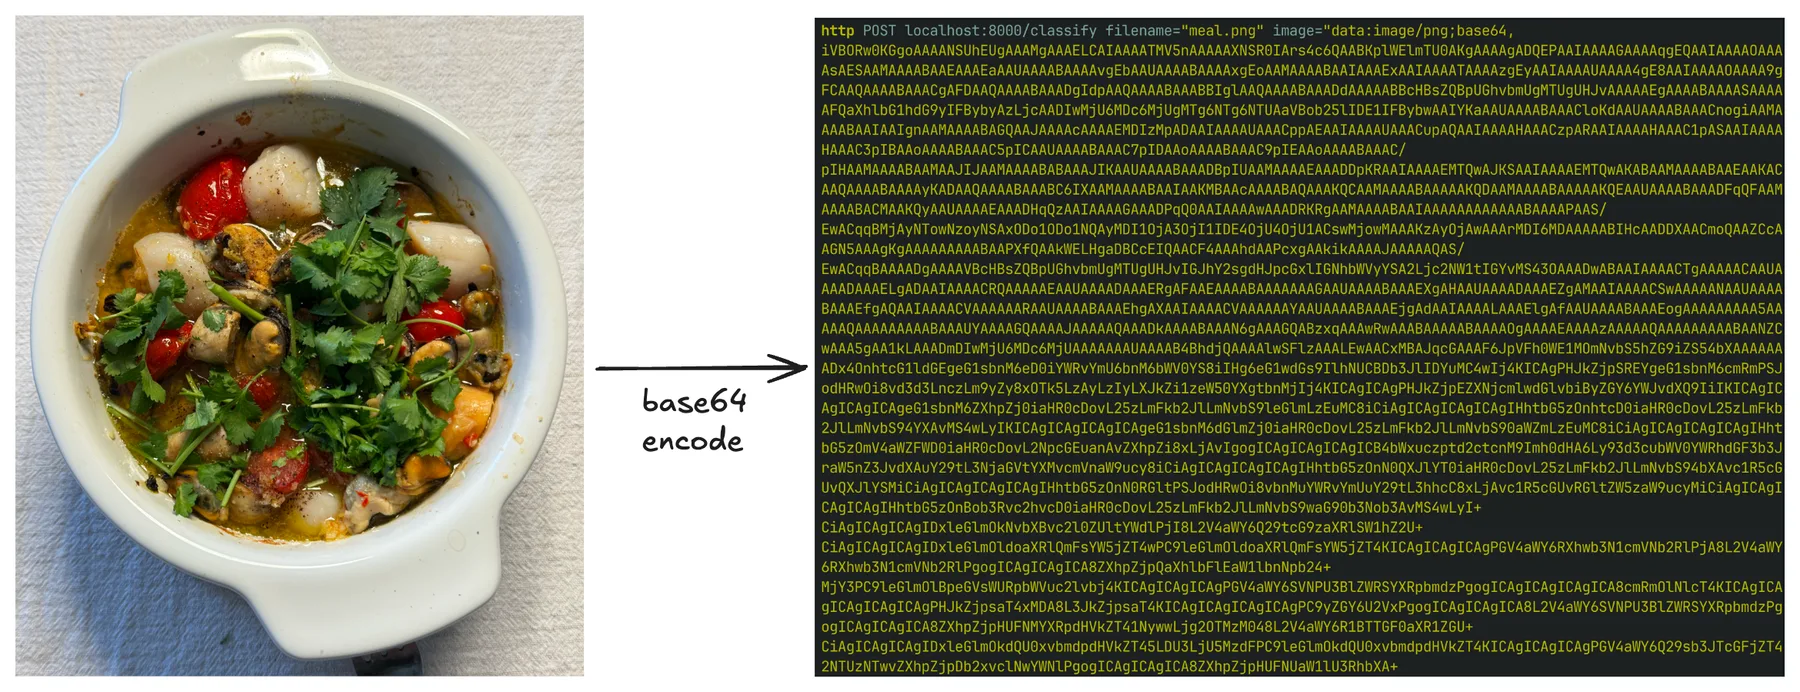
\includegraphics[width=0.8\textwidth]{seafood-casserole}
        \end{center}
    \end{figure}

    \vspace{-0.5em}
    Top predictions: soup bowl (0.57), consomme (0.22), hot pot (0.16), mortar (0.01), potpie (0.01).
\end{frame}


\section{Going Async}

\begin{frame}{Two awkward properties}
    The server above works but has two awkward properties, each with a solution.

    \begin{block}{1. The model is loaded at the top of the file}
\begin{itemize}
\item Every Uvicorn auto-reload during development triggers a fresh download check and a few hundred megabytes of disk reads
\item Before the model is downloaded and loaded, the server cannot process any incoming requests
\item Solvable using the \texttt{lifespan} context manager
\end{itemize}
    \end{block}

    \begin{block}{2. Every request runs in a regular synchronous function}
\begin{itemize}
\item While one request is being processed, the server essentially freezes and cannot process any other incoming requests
\item Solvable using the \texttt{async} endpoints
\end{itemize}
    \end{block}
\end{frame}

\begin{frame}[fragile]{Loading the model once at startup}
    \texttt{lifespan} is an async context manager attached to the FastAPI app.
    The code before \texttt{yield} runs once when the server starts, and the code after \texttt{yield} runs once when it shuts down.

    \begin{minted}{python}
from contextlib import asynccontextmanager
ml = {}

@asynccontextmanager
async def lifespan(app: FastAPI):
    weights = ResNet18_Weights.DEFAULT
    model = resnet18(weights=weights); model.eval()
    ml["model"] = model
    ml["preprocess"] = weights.transforms()
    ml["categories"] = weights.meta["categories"]
    yield
    ml.clear()

app = FastAPI(lifespan=lifespan)
    \end{minted}
\end{frame}

\begin{frame}{The waiter analogy}
A useful way to think about \texttt{async} functions is to imagine an endpoint as \textbf{a single waiter at a busy restaurant}.

    \begin{block}{Without \texttt{async}}
        The waiter takes one order, walks to the kitchen, stands there until the food is ready, then walks it back to the table before taking the next order.
        Most of the time the waiter just stands around.
    \end{block}

    \begin{block}{With \texttt{async}}
After handing the order to the kitchen, the waiter immediately moves on to take other tables' orders, and only comes back to deliver the food once the kitchen says it is ready. \textit{Suppose there are cooks in the kitchen.}
    \end{block}
\end{frame}

\begin{frame}[fragile]{Async endpoint with \texttt{asyncio.to\_thread}}
    For our classification endpoint, the slow part is the model inference itself.
    The waiter will be busy cooking the food, thus marking the endpoint \texttt{async} alone does not help.
    The fix is to hire a separate cook. We hand the inference call to another thread.

    \begin{minted}{python}
import asyncio

@app.post("/v1/classify")
async def classify(req: ImageRequest):
    image = decode_image(req.image)
    predictions = await asyncio.to_thread(run_inference, image)
    return {"model": "resnet18", "predictions": predictions}
    \end{minted}

The endpoint is \texttt{async}, plus the heavy work runs in a separate thread.
While the inference thread runs, the server keeps accepting other requests.
\end{frame}

\begin{frame}{When async really pays off}
    \texttt{async} and \texttt{await} are useful when the endpoint mostly waits on something external.
For example, calling another remote AI API, or querying a database.

\begin{enumerate}
\item Use \texttt{async} and \texttt{await} when the endpoint waits on the outside world.
\item Add \texttt{asyncio.to\_thread} to offload heavy computation done internally.
\end{enumerate}
\end{frame}


\section{Protecting the Endpoints}

\begin{frame}{Why protect the endpoints}
    So far our server happily serves anyone who knows its address.
    Fine for local development.
The moment we put it on the internet, \textit{anyone can poke at it}.

    \begin{figure}[htpb]
        \begin{center}
            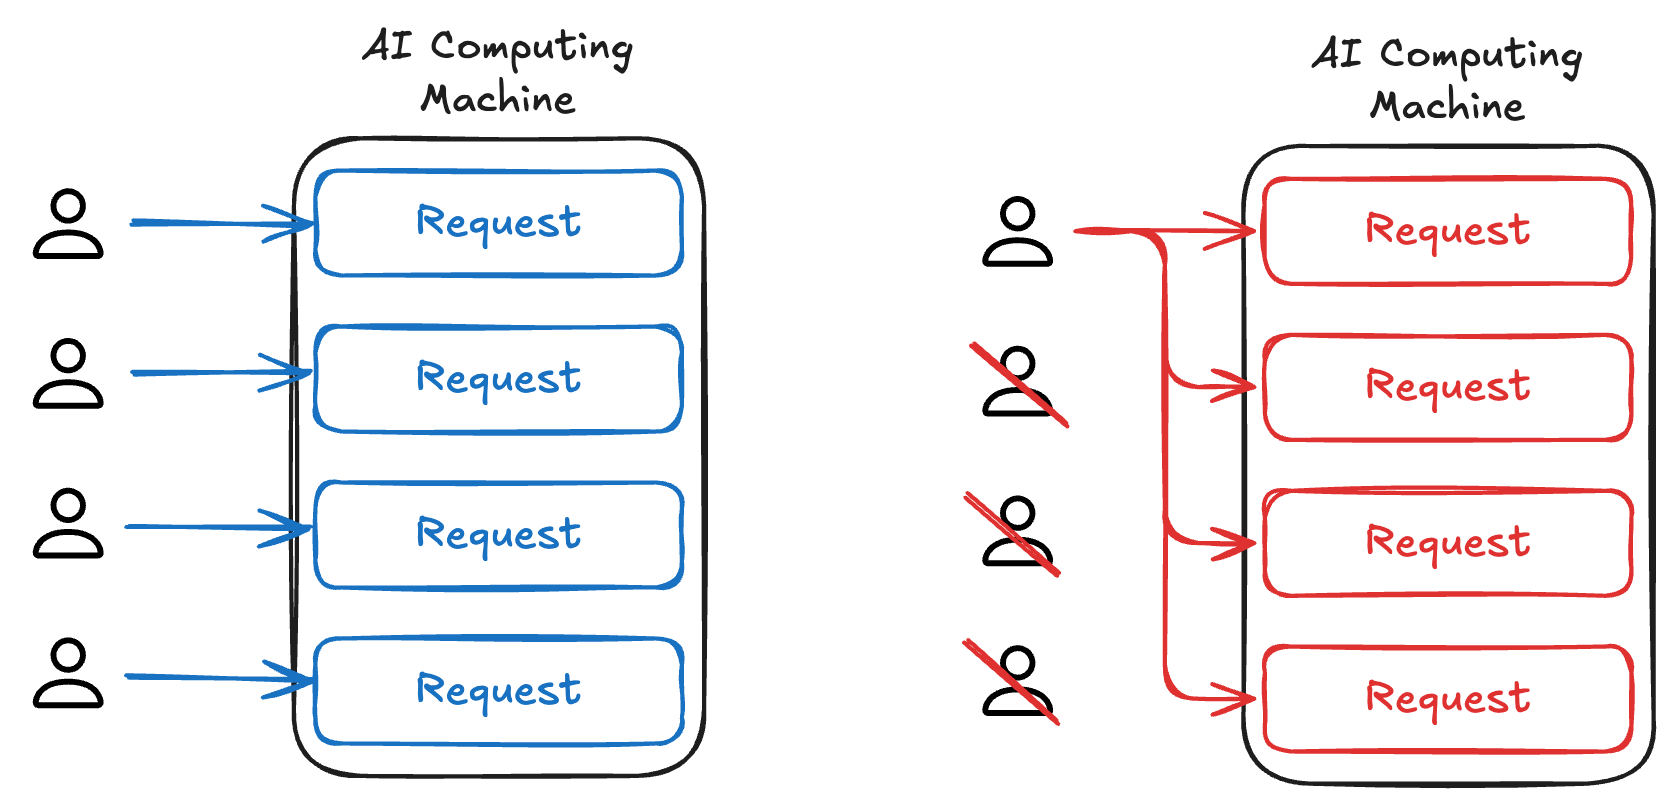
\includegraphics[width=0.55\textwidth]{bad_actors}
        \end{center}
    \end{figure}

\textit{AI inference is expensive}. An unprotected endpoint can be used to overload our hardware or run up our cloud or electricity bill within minutes.
\end{frame}

\begin{frame}{Three protections most real AI APIs have}
    \begin{enumerate}
        \item \textbf{API key authentication.} Identify the caller
        \item \textbf{Per-user usage tracking.} Record who called and when
        \item \textbf{Rate limiting.} Cap how often each user can call us
    \end{enumerate}
\end{frame}

\begin{frame}[fragile]{API key auth, hardcoded version}
    Same shape as OpenAI: \texttt{Authorization: Bearer <key>}.

    \begin{minted}{python}
from fastapi import Depends, HTTPException, status
from fastapi.security import HTTPBearer, HTTPAuthorizationCredentials

bearer_scheme = HTTPBearer()
VALID_API_KEYS = {"sk-mysecretkey-001", "sk-mysecretkey-002"}

def verify_api_key(
    creds: HTTPAuthorizationCredentials = Depends(bearer_scheme),
) -> str:
    if creds.credentials not in VALID_API_KEYS:
        raise HTTPException(401, "Invalid API key")
    return creds.credentials
    \end{minted}

    Add it as a dependency on any endpoint to require auth.
\end{frame}

\begin{frame}[fragile]{Putting it on the endpoint}
    \begin{minted}{python}
@app.post("/v1/classify")
async def classify(
    req: ImageRequest,
    api_key: str = Depends(verify_api_key),
):
    ...
    \end{minted}

    \vspace{0.5em}
    \begin{itemize}
        \item Missing or invalid \texttt{Authorization} header: \texttt{401 Unauthorized} before the model runs
        \item Valid header: function gets the key and proceeds
    \end{itemize}

    Hardcoded keys are fine for one or two users, but useless beyond that.
\end{frame}

\begin{frame}[fragile]{Moving keys into a database}
To dynamically manage the list of valid API keys, we should integrate a \textbf{database}.
SQLite plus SQLAlchemy is enough for a small server.

    \begin{minted}{python}
class User(Base):
    __tablename__ = "users"
    id: Mapped[int] = mapped_column(primary_key=True)
    api_key: Mapped[str] = mapped_column(unique=True)
    \end{minted}

\end{frame}

\begin{frame}[fragile]{Looking up the key in the database}
    \begin{minted}{python}
def get_current_user(
    creds: HTTPAuthorizationCredentials = Depends(bearer_scheme),
    db: Session = Depends(get_session),
) -> User:
    user = db.scalar(select(User).where(User.api_key == creds.credentials))
    if user is None:
        raise HTTPException(401, "Invalid API key")
    return user

@app.post("/v1/classify")
async def classify(req: ImageRequest,
                   user: User = Depends(get_current_user),
                   db: Session = Depends(get_session)):
    ...
    \end{minted}

    Update the database to add or revoke keys, rather than change the code and redeploy.
\end{frame}

\begin{frame}[fragile]{Logging each request}
Database integration also makes it easy to record per-user usage.
Prepare a table for recording each request...

    \begin{minted}{python}
class User(Base):
    __tablename__ = "users"
    id: Mapped[int] = mapped_column(primary_key=True)
    api_key: Mapped[str] = mapped_column(unique=True)
    requests: Mapped[list["APIRequest"]] = relationship(back_populates="user")

class APIRequest(Base):
    __tablename__ = "api_requests"
    id: Mapped[int] = mapped_column(primary_key=True)
    user_id: Mapped[int] = mapped_column(ForeignKey("users.id"))
    timestamp: Mapped[datetime] = mapped_column(default=datetime.utcnow)
    \end{minted}
\end{frame}


\begin{frame}[fragile]{Logging each request}
...and insert a database entry every time a request is processed.

    \begin{minted}{python}
@app.post("/v1/classify")
async def classify(req, user=Depends(get_current_user), db=Depends(get_session)):
    start = time.perf_counter()
    status_code = 200
    try:
        ...  # normal classification
        return result
    except HTTPException as e:
        status_code = e.status_code
        raise
    finally:
        db.add(APIRequest(user_id=user.id))
        db.commit()
    \end{minted}

\end{frame}


\section{Rate Limiting}

\begin{frame}{Why rate limit}
    Even with API keys in place, a misbehaving or malicious client can send thousands of requests per minute and overload the server.

    \begin{figure}[htpb]
        \begin{center}
            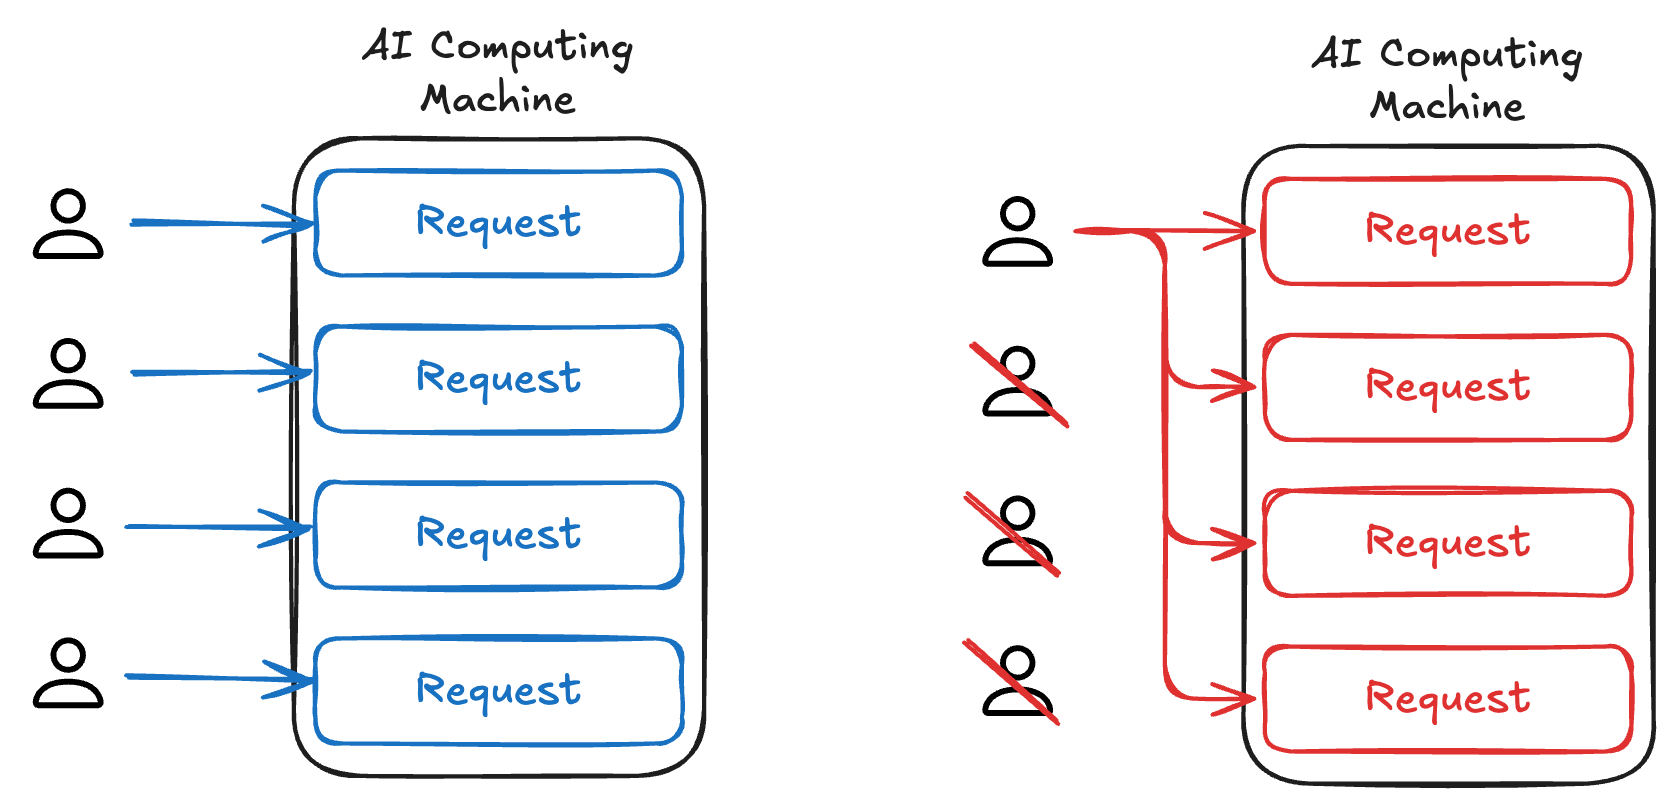
\includegraphics[width=0.55\textwidth]{bad_actors}
        \end{center}
    \end{figure}

    \vspace{0.5em}
    A rate limit caps the number of requests each user can make in a given time window.
Two algorithms are commonly used: \textbf{fixed window} and \textbf{sliding window}.
\end{frame}

\begin{frame}{Fixed window}
\textbf{Divides time into fixed intervals}, say every minute on the minute.
    Each interval has a counter that resets to zero at the boundary.

    \begin{figure}[htpb]
        \begin{center}
            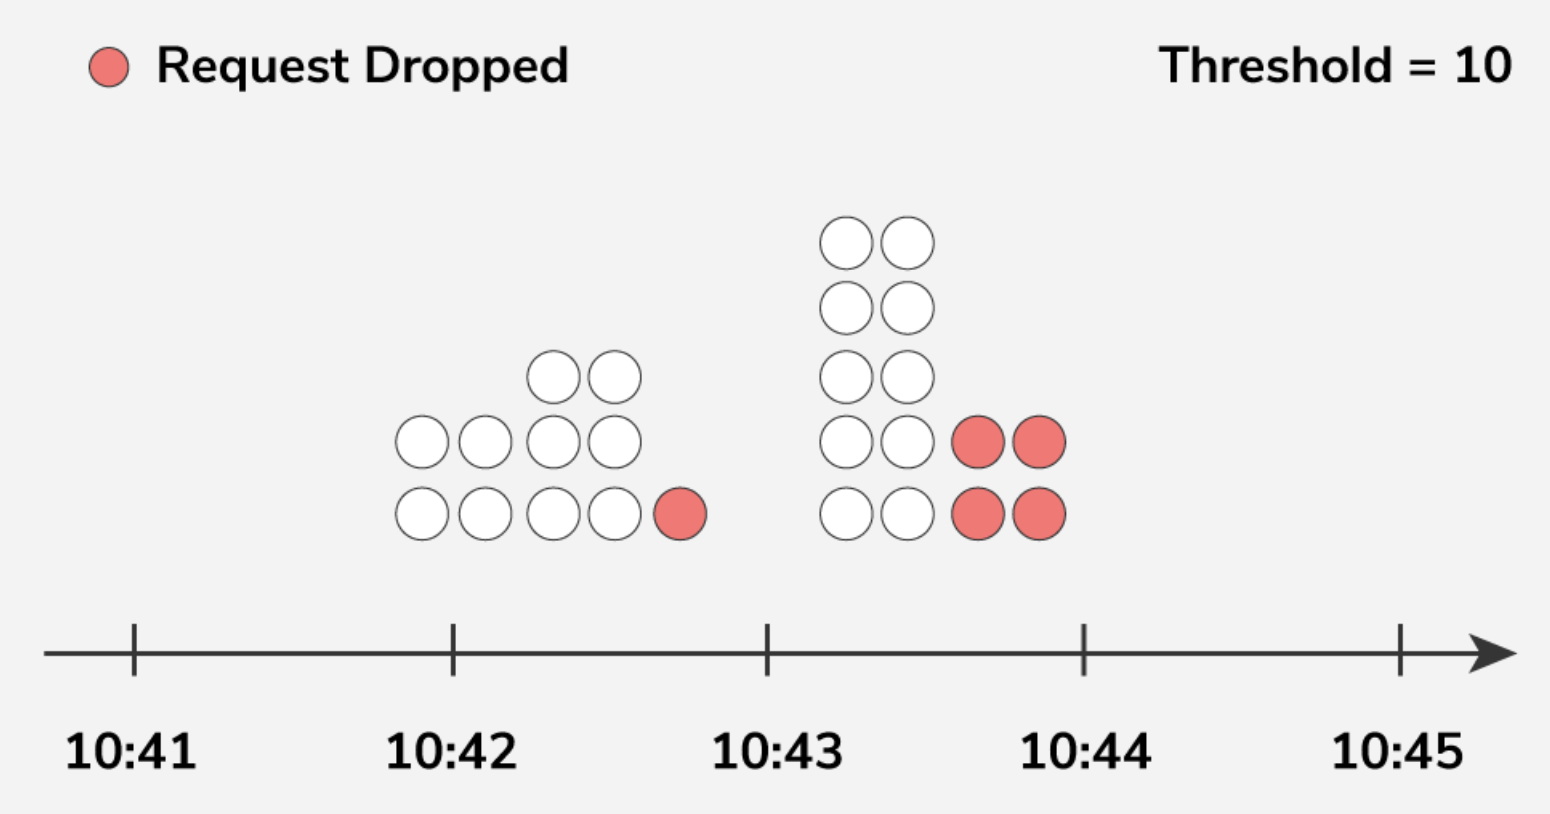
\includegraphics[width=0.5\textwidth]{rl_fixed_window}
        \end{center}
    \end{figure}

    Simple to implement.
However, it lets a client send \textit{a burst of \texttt{2 * limit} requests around the boundary}, by squeezing in \texttt{limit} requests just before the window flips and another \texttt{limit} immediately after.
\end{frame}

\begin{frame}{Sliding window}
Looks at the last \texttt{N} seconds \textbf{from the current moment}.
    At every request, count how many the user has made in the past \texttt{N} seconds, reject if the count exceeds the limit.

    \begin{figure}[htpb]
        \begin{center}
            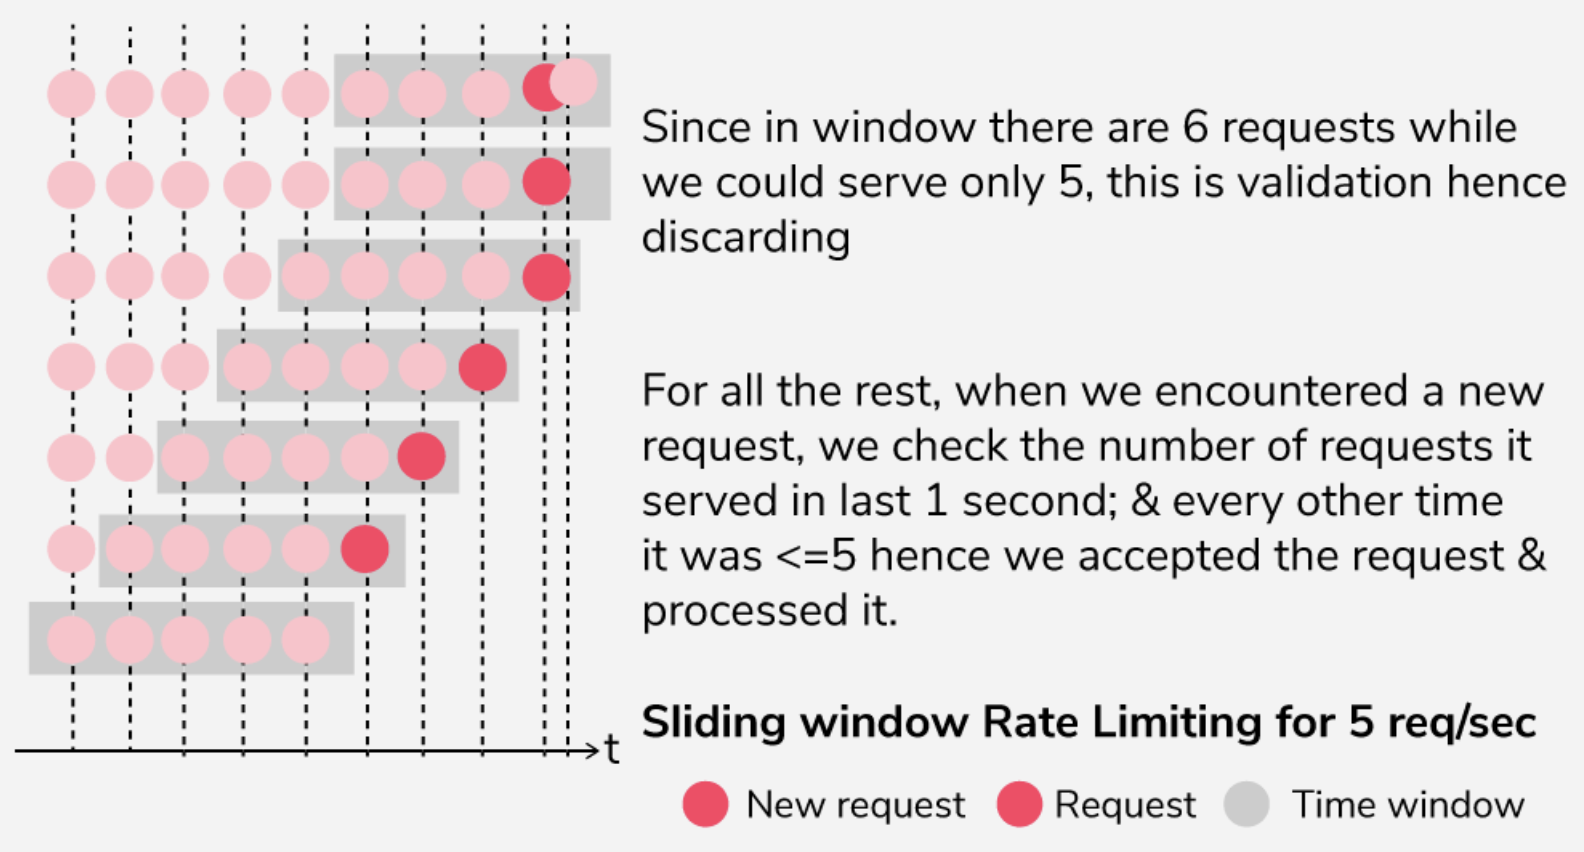
\includegraphics[width=0.5\textwidth]{rl_sliding_window}
        \end{center}
    \end{figure}

\textbf{Smoother} and avoids the burst at the boundary, at the cost of having to look up recent requests at each call.
\end{frame}

\begin{frame}[fragile]{Example: sliding window implementation}
Any rate limit algorithm requires recording every request into a database.

    \begin{minted}{python}
from datetime import datetime, timedelta, timezone

RATE_LIMIT = 5
WINDOW_SECONDS = 60

def check_rate_limit(user: User, db: Session):
    cutoff = datetime.now(timezone.utc) - timedelta(seconds=WINDOW_SECONDS)
    recent = db.scalar(
        select(func.count()).select_from(APIRequest)
        .where(APIRequest.user_id == user.id,
               APIRequest.timestamp >= cutoff)
    )
    if recent >= RATE_LIMIT:
        raise HTTPException(429, "Rate limit exceeded")
    \end{minted}

    One call at the start of the endpoint, and a flurry of requests returns \texttt{429 Too Many Requests}.
\end{frame}


\section{Exercise}

\begin{frame}{Bring your server to life}
    Take the A.3 server and make it actually compute with a real AI model.

    \begin{block}{Outline}
        \begin{enumerate}
            \item Pick a model that runs on your hardware (ResNet-18 if CPU only, anything bigger if you have a GPU)
            \item Load it once with \texttt{lifespan}, confirm it loads only once on auto-reload
            \item Replace the hardcoded response in \texttt{/v1/classify} with a real inference call, offloaded AI compute via \texttt{asyncio.to\_thread}
            \item Point the A.2 program at it and watch real predictions come back
        \end{enumerate}
    \end{block}
\end{frame}

\begin{frame}{Extensions}
    \begin{enumerate}
        \item Add API key auth backed by SQLite, log every request
        \item Add a sliding-window rate limit with a low cap (e.g., 5 per minute), then send a burst of requests from the A.2 program and watch \texttt{429}s come back
        \item If you have a real LLM available, build \texttt{/v1/chat/stream} that forwards an SSE stream from the model
    \end{enumerate}
\end{frame}

\begin{frame}{What you should walk away with}
    By the end of the exercise, you should be able to:
    \begin{enumerate}
        \item Understand how AI models are integrated into API servers
        \item Know common FastAPI practices in an AI-enabled API server
        \item Design and implement an AI API server that behaves like a real one
    \end{enumerate}

    \vspace{0.5em}
By the end of Part A, you should be able to design and implement a closed-loop AI system, including the client and server programs.

    \vspace{0.5em}
In Part B, we will learn how to deploy this system onto diverse real-world infrastructure.
\end{frame}


\appendix

\begin{frame}[plain,noframenumbering]
\begin{center}
{\large Thank you!}
\vspace{1cm}
\\[0.5em]
{\small \faEnvelope\ \href{mailto:lyan@cs.aau.dk}{lyan@cs.aau.dk} \\
\faGlobe\ \href{https://www.yanlincs.com}{www.yanlincs.com}}
\end{center}
\end{frame}

\end{document}
